%%%%%%%%%%%%%%%%%%%%%%%%%%%%%%%%%%%%%%%%%%%%%%%%%%%%%%%%%%%%%%%%%%%%%%%%%%%

\chapter{Vectors and Matrices}


%%%%%%%%%%%%%%%%%%%%%%%%%%%%%%%%%%%%%%%%%%%%%%%%%%%%%%%%%%%%%%%%%%%%%%%%%%%

\section{Scalars and vectors}
\label{sec:scalars_vectors}
\index{scalar}
\index{two-dimensional vectors}
\index{vector}

The path of a car travelling from location $A$ to location $B$ is
characterized by two quantities or \emph{scalars}\index{scalars}: a
magnitude\index{magnitude}~(such as speed), and a direction~(from $A$
to $B$). Both of these two scalars are summarized by a
\emph{vector}\index{vector}.

\begin{figure}[!htpb]
\centering
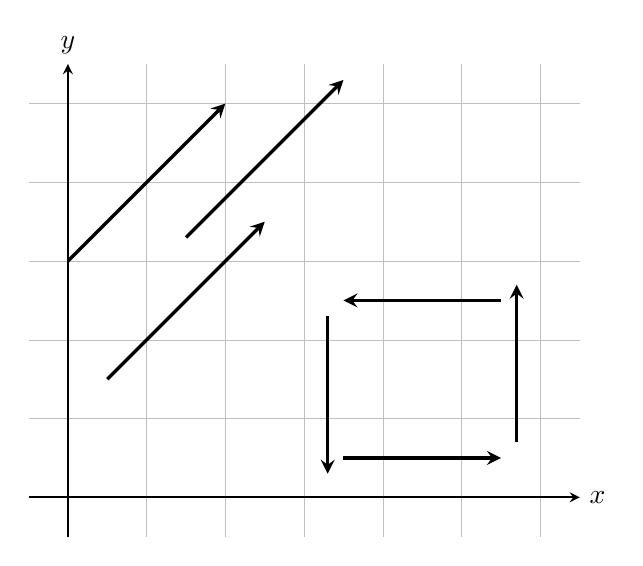
\begin{tikzpicture}
[linedecorate/.style={->,>=stealth,very thick}]
% grids for the plane
\draw[step=1cm,lightgray,very thin] (-0.5,-0.5) grid (6.5,5.5);
% the rectangular axes
\draw[->,>=stealth,semithick] (-0.5,0) -- (6.5,0) node[right]{$x$};
\draw[->,>=stealth,semithick] (0,-0.5) -- (0,5.5) node[above]{$y$};
% vectors
\draw[linedecorate] (0,3) -- node[above left]{$\vecu$} (2,5);
\draw[linedecorate] (1.5,3.3) -- node[below right]{$\vecv$} (3.5,5.3);
\draw[linedecorate] (0.5,1.5) -- node[below right]{$\vecw$} (2.5,3.5);
\draw[linedecorate] (3.5,0.5) -- (5.5,0.5);
\draw[linedecorate] (5.7,0.7) -- (5.7,2.7);
\draw[linedecorate] (5.5,2.5) -- (3.5,2.5);
\draw[linedecorate] (3.3,2.3) -- (3.3,0.3);
\end{tikzpicture}
\caption{Vectors in the $x$-$y$ plane.}
\label{fig:vectors_matrices:plane_vectors}
\end{figure}

In the $x$-$y$ plane, we can visualize a vector as an arrow from point
$A$ to point $B$~(see
Figure~\ref{fig:vectors_matrices:plane_vectors}). The starting point
$A$ of the vector is called the
\emph{tail}\index{vector!tail}\index{tail} and the terminal point $B$
is the \emph{head}\index{vector!head}\index{head}. Two vectors are
\emph{equivalent}\index{vector!equivalent} if they have the same
magnitude and direction. The vectors $\vecu$, $\vecv$, and $\vecw$ in
Figure~\ref{fig:vectors_matrices:plane_vectors} are thus all
equivalent to each other.

To analyze vectors using algebra, we can think of a vector $\vecu$
as starting from the origin of the $x$-$y$ plane and having
$(u_1, u_2)$ as the coordinate for its head~(see
Figure~\ref{fig:specify_vector_head_coordinate}). So $\vecu$ is
completely determined by the coordinate of its head and we write
$\vecu = \langle u_1, u_2 \rangle$ as an algebraic representation
for $\vecu$.

\begin{figure}[!htpb]
\centering
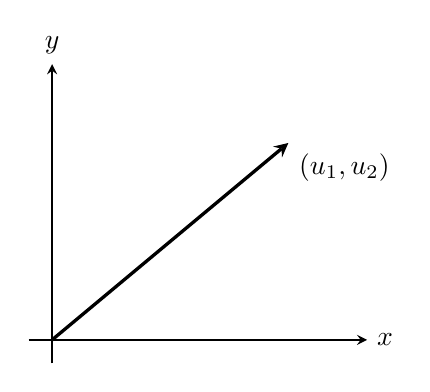
\begin{tikzpicture}
% the rectangular axes
\draw[->,>=stealth,semithick] (-0.3,0) -- (4,0) node[right]{$x$};
\draw[->,>=stealth,semithick] (0,-0.3) -- (0,3.5) node[above]{$y$};
% vector described by its head coordinate
\draw[->,>=stealth,very thick] (0,0) -- node[above left]{$\vecu$} (3,2.5) node[below right]{$(u_1, u_2)$};
\end{tikzpicture}
\caption{A vector as specified by its head coordinate.}
\label{fig:specify_vector_head_coordinate}
\end{figure}

In case the tail\index{vector!tail}\index{tail} of $\vecu$ is not the
origin, we let $(x_1, y_1)$ be the coordinate of the tail and denote
the coordinate of the head by $(x_2, y_2)$. By subtracting
coordinatewise, we obtain an equivalent vector $\vecv$ that emanates
from the origin of the $x$-$y$ plane. The coordinate of $\vecv$ is
\[
(x_2, y_2) - (x_1, y_1)
=
(x_2 - x_1,\; y_2 - y_1)
=
(u_1, u_2)
\]
and we do not distinguish between $\vecu$ and $\vecv$. Thus we
can transform $\vecu$ to be a vector emanating from the origin and
specified by the coordinate
%
\begin{equation}
\label{eq:component_form_vector}
\vecu
=
\langle x_2 - x_1,\; y_2 - y_1 \rangle
=
\langle u_1, u_2 \rangle.
\end{equation}
%
Equation~(\ref{eq:component_form_vector}) is called the
\emph{component form}\index{component form} of a vector, with $u_1$
and $u_2$ being the individual components. The vector
$\veczero = \langle 0, 0 \rangle$ is called the zero
vector\index{zero vector}.

\begin{figure}[!htpb]
\centering
\begin{tikzpicture}
% the rectangular axes
\draw[->,>=stealth,semithick] (-2.5,0) -- (5.7,0) node[right]{$x$};
\draw[->,>=stealth,semithick] (0,-1.5) -- (0,6.7) node[above]{$y$};
% ticks on horizontal axis
\foreach \x in {-2,-1,-1}
  \draw (\x cm,2pt) -- (\x cm,-2pt) node[anchor=north] {$\x$};
\foreach \x in {1,2,...,5}
  \draw (\x cm,2pt) -- (\x cm,-2pt) node[anchor=north] {$\x$};
% ticks on vertical axis
\foreach \y in {-1,-1}
  \draw (2pt,\y cm) -- (-2pt,\y cm) node[anchor=east] {$\y$};
\foreach \y in {1,2,...,6}
  \draw (2pt,\y cm) -- (-2pt,\y cm) node[anchor=east] {$\y$};
% vector u
\draw[->,>=stealth,very thick] (-2,-1) node[below]{$(-2,-1)$} -- node[above left]{$\vecu$} (1,3) node[above]{$(1,3)$};
% vector v
\draw[->,>=stealth,very thick] (1.5,1.5) node[below]{$(1.5,1.5)$} -- node[above left]{$\vecv$} (4.5,5.5) node[above]{$(4.5,5.5)$};
\end{tikzpicture}
\caption{Verify that vectors $\vecu$ and $\vecv$ are equivalent.}
\label{fig:vectors_matrices:verify_vectors_u_v}
\end{figure}

\begin{example}
Let the vector $\vecu$ be described by the directed line segment
from $(-2,-1)$ to $(1,3)$, and let $\vecv$ be the line segment from
$(1.5,1.5)$ to $(4.5,5.5)$, as shown in
Figure~\ref{fig:vectors_matrices:verify_vectors_u_v}. Show that
$\vecu$ and $\vecv$ are equivalent vectors.
\end{example}

\begin{proof}[Solution]
To show that $\vecu$ and $\vecv$ are equivalent, we need to show
that they have the same length and are in the same direction. The
length of $\vecu$ is equivalent to the length of the line segment
from $(-2,-1)$ to $(1,3)$:
%
\begin{align*}
\sqrt{(1 - (-2))^2 + (3 - (-1))^2}
&=
\sqrt{(1 + 2)^2 + (3 + 1)^2} \\
&=
\sqrt{9 + 16} \\
&=
5.
\end{align*}
%
This tells us that $\vecu$ has length 5. Similarly, the length of
$\vecv$ is
%
\begin{align*}
\sqrt{(4.5 - 1.5)^2 + (5.5 - 1.5)^2}
&=
\sqrt{3^2 + 4^2} \\
&=
\sqrt{9 + 16} \\
&=
5
\end{align*}
%
which is the same length as that of $\vecu$.

\begin{lstlisting}
sage: u = vector([1 - (-2), 3 - (-1)]); u
(3, 4)
sage: v = vector([4.5 - 1.5, 5.5 - 1.5]); v
(3.000...000, 4.000...000)
sage: u.norm()
5
sage: v.norm()
5.000...000
\end{lstlisting}

The slope\index{slope}\index{gradient} of the line segment from
$(-2,-1)$ to $(1,3)$ is
\[
\frac{3 - (-1)} {1 - (-2)}
=
\frac{4}{3}
\]
and the slope of the line segment from $(1.5,1.5)$ to $(4.5,5.5)$ is
\[
\frac{5.5 - 1.5}{4.5 - 1.5}
=
\frac{4}{3}
\]
which shows that these two line segments have the same direction, so
$\vecu$ and $\vecv$ point in the same direction.
%
\begin{lstlisting}
sage: (3 - (-1)) / (1 - (-2))
4/3
sage: (5.5 - 1.5) / (4.5 - 1.5)
1.333...333
sage: QQ((5.5 - 1.5) / (4.5 - 1.5))
4/3
\end{lstlisting}
%
Therefore, $\vecu$ and $\vecv$ are equivalent vectors.
\end{proof}

We denote the length\index{vector!length}\index{length} of a vector as
follows. Let $\vecu$ be a vector whose starting point is
$P = (x_1, y_1)$ and whose terminal point is $Q = (x_2, y_2)$. Then
the \emph{length} or
\emph{magnitude}\index{vector!magnitude}\index{magnitude} of $\vecu$
is denoted by $\vecvertl \vecu \vecvertr$ and given by the equation
%
\begin{equation}
\label{eq:vectors_matrices:magnitude_two_dimensional_vector}
\begin{aligned}
\vecvertl \vecu \vecvertr
&=
\sqrt{(x_2 - x_1)^2 + (y_2 - y_1)^2} \\
&=
\sqrt{v_1^2 + v_2^2}.
\end{aligned}
\end{equation}


%%%%%%%%%%%%%%%%%%%%%%%%%%%%%%%%%%%%%%%%%%%%%%%%%%%%%%%%%%%%%%%%%%%%%%%%%%%

\section{Add, subtract, and multiply vectors}
\index{vector!arithmetic}

The left-hand side of Figure~\ref{fig:vectors_matrices:vector_sum}
illustrates the path of an object. Initially travelling in the
direction of vector $\vecu$, the object then changes its direction to
move in the direction of $\vecv$. The total displacement of the object
is represented as the vector $\vecu + \vecv = \vecw$. Furthermore, we
could first go in the direction of $\vecv$ and then in that of $\vecu$,
and hence obtain the same displacement $\vecv + \vecu = \vecw$, as
shown on the right-hand side of
Figure~\ref{fig:vectors_matrices:vector_sum}. This ``adding'' of
vectors is just one of many basic operations that can be performed on
vectors. In fact, the ``adding'' rule illustrated in
Figure~\ref{fig:vectors_matrices:vector_sum} is called the
\emph{parallelogram rule}\index{parallelogram rule} for vector
addition.

\begin{figure}[!htpb]
\centering
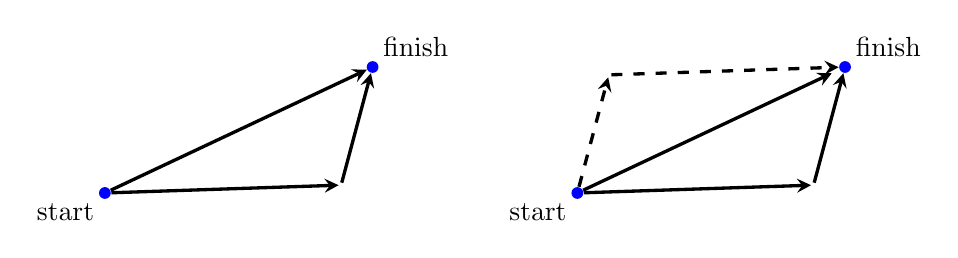
\begin{tikzpicture}
% left set of vectors
\node (start1) at (0,0) [circle,fill=blue,inner sep=1.5pt]{};
\node (middle1) at (3,0.1) [circle,inner sep=0.5pt]{};
\node (finish1) at (3.4,1.6) [circle,fill=blue,inner sep=1.5pt]{};
\draw[->,>=stealth,very thick] (start1) node[below left]{start}  -- node[below]{$\vecu$} (middle1);
\draw[->,>=stealth,very thick] (middle1) -- node[right]{$\vecv$} (finish1) node[above right]{finish};
\draw[->,>=stealth,very thick] (start1) -- node[above]{$\vecw$} (finish1);
% right set of vectors
\node (start2) at (6,0) [circle,fill=blue,inner sep=1.5pt]{};
\node (lowerMiddle) at (9,0.1) [circle,inner sep=0.5pt]{};
\node (upperMiddle) at (6.4,1.5) [circle,inner sep=0.5pt]{};
\node (finish2) at (9.4,1.6) [circle,fill=blue,inner sep=1.5pt]{};
\draw[->,>=stealth,very thick] (start2) node[below left]{start} -- node[below]{$\vecu$} (lowerMiddle);
\draw[->,>=stealth,very thick] (lowerMiddle) -- node[right]{$\vecv$} (finish2) node[above right]{finish};
\draw[->,>=stealth,shorten >=3pt,very thick] (start2) -- node[above]{$\vecw$} (finish2);
\draw[->,>=stealth,very thick,dash pattern=on 4pt off 4pt] (start2) -- node[left]{$\vecv$} (upperMiddle);
\draw[->,>=stealth,very thick,dash pattern=on 4pt off 4pt] (upperMiddle) -- node[above]{$\vecu$} (finish2);
\end{tikzpicture}
\caption{The vector sum $\vecu + \vecv = \vecw = \vecv + \vecu$.}
\label{fig:vectors_matrices:vector_sum}
\end{figure}

\begin{definition}
\label{def:vectors_matrices:vector_operations}
\index{vector!arithmetic}
Let $\vecu = \langle u_1, u_2 \rangle$ and
$\vecv = \langle v_1, v_2 \rangle$ be vectors and suppose
$c$ is a scalar. Then we have the following operations on vectors:
\begin{enumerate}
\item The \emph{vector sum}\index{sum} of $\vecu$ and
  $\vecv$ is $\vecu + \vecv = \langle u_1 + v_1,\; u_2 + v_2 \rangle$.

\item The \emph{negative}\index{negative} of $\vecu$ is
  $-\vecu = \langle -u_1, -u_2 \rangle$.

\item The \emph{vector difference}\index{difference} of $\vecu$ and
  $\vecv$ is $\vecu - \vecv =
  \langle u_1, u_2 \rangle - \langle v_1, v_2 \rangle = \langle u_1 -
  v_1,\; u_2 - v_2 \rangle$.

\item The \emph{scalar multiple}\index{scalar multiple} of $c$ and
  $\vecu$ is $c\vecu = \langle c u_1, c u_2 \rangle$.
\end{enumerate}
\end{definition}

The negative of a vector $\vecu$ is a vector that has the same
length as $\vecu$, but goes in the opposite direction. One
exception is the zero vector $\veczero$, whose negative is itself
because $-\veczero = -\langle 0,0 \rangle = \langle -0, -0 \rangle =
\langle 0,0 \rangle = \veczero$. More generally, scalar
multiplication has the effect of scaling a vector. This may result in
expanding the vector, contracting it, producing the negative of the
vector, or expanding/contracting the negative of the vector. These
various possibilities are shown in
Figure~\ref{fig:scalar_multiply_negative}.

\begin{figure}[!htpb]
\centering
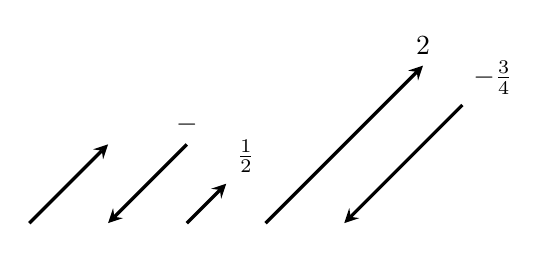
\begin{tikzpicture}
\draw[->,>=stealth,very thick] (0,0) -- (1,1) node[above]{$\vecu$};
\draw[<-,>=stealth,very thick] (1,0) -- (2,1) node[above]{$-\vecu$};
\draw[->,>=stealth,very thick] (2,0) -- (2.5,0.5) node[above right]{$\frac{1}{2}\vecu$};
\draw[->,>=stealth,very thick] (3,0) -- (5,2) node[above]{$2\vecu$};
\draw[<-,>=stealth,very thick] (4,0) -- (5.5,1.5) node[above right]{$-\frac{3}{4}\vecu$};
\end{tikzpicture}
\caption{Scalar multiplication and negative of a vector.}
\label{fig:scalar_multiply_negative}
\end{figure}

Using the parallelogram rule\index{parallelogram rule} for vector
addition, we can similarly illustrate vector difference. The left-hand
side of
Figure~\ref{fig:vectors_matrices:vector_difference_parallelogram_triangle}
shows the parallelogram rule for vector subtraction, while the
right-hand side shows the triangle rule for vector subtraction. Thus
to determine the difference of two vectors $\vecu$ and $\vecv$, we
first align the vectors so that their initial points coincide. Then
the difference $\vecu - \vecv$ is the vector that starts from the head
of $\vecv$ and ends at the terminal point of $\vecu$.

\begin{figure}[!htpb]
\centering
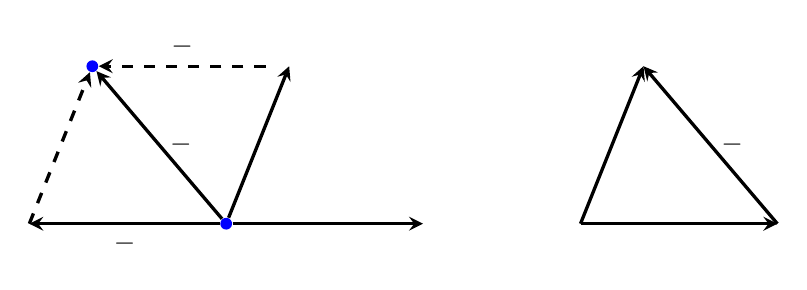
\begin{tikzpicture}
% left-hand figure: vector difference by parallelogram rule
\node (origin) at (0,0) [circle,fill=blue,inner sep=1.5pt]{};
\node (destin) at (-1.7,2) [circle,fill=blue,inner sep=1.5pt]{};
\draw[->,>=stealth,very thick] (origin) -- node[below]{$\vecv$} (2.5,0);
\draw[->,>=stealth,very thick] (origin) -- node[below]{$-\vecv$} (-2.5,0);
\draw[->,>=stealth,very thick] (origin) -- node[right]{$\vecu$} (0.8,2);
\draw[->,>=stealth,very thick,dash pattern=on 4pt off 4pt] (-2.5,0) -- node[left]{$\vecu$} (destin);
\draw[->,>=stealth,very thick,dash pattern=on 4pt off 4pt] (0.5,2) -- node[above]{$-\vecv$} (destin);
\draw[->,>=stealth,very thick] (origin) -- node[right]{$\vecu - \vecv$} (destin);
% right-hand figure: vector difference
\draw[->,>=stealth,very thick] (4.5,0) -- node[left]{$\vecu$} (5.3,2);
\draw[->,>=stealth,very thick] (4.5,0) -- node[below]{$\vecv$} (7,0);
\draw[->,>=stealth,very thick] (7,0) -- node[right]{$\vecu - \vecv$} (5.3,2);
\end{tikzpicture}
\caption{Vector difference by the parallelogram rule~(left) and by the
triangle rule~(right).}
\label{fig:vectors_matrices:vector_difference_parallelogram_triangle}
\end{figure}

Vector operations share many of the familiar properties of operations
on real numbers. Given two real numbers, for example, it does not
matter in which order we add
them. Problem~\ref{prob:vectors_matrices:field_laws_for_vectors} lists
a number of vector rules that are similar to those obeyed by real numbers.

\begin{example}
Using vector rules from
problem~\ref{prob:vectors_matrices:field_laws_for_vectors}, find a
vector $\vecx$ such that $5\vecx + 7\vecu = 4\vecv$.
\end{example}

\begin{proof}[Solution]
First, subtract $7\vecu$ from both sides of the equal sign to get
$5\vecx + (7\vecu - 7\vecu) = 4\vecv - 7\vecu$, which can be
simplified to $5\vecx = 4\vecv - 7\vecu$. Now divide both sides of
the last equation by $5$ and we have
$\frac{1}{5} (5\vecx) = \frac{1}{5} (4\vecv - 7\vecu)$. Simplify the
last equation to
$\vecx = \frac{1}{5} (4\vecv) + \frac{1}{5}(-7\vecu)$. So the required
vector is $\vecx = \frac{4}{5}\vecv - \frac{7}{5}\vecu$.
\end{proof}

Any nonzero vector $\vecv$ can be transformed into a vector $\vecu$ of
magnitude $1$\index{unit vector}. The equation to effect this
transformation is
%
\begin{equation}
\label{eq:vectors_matrices:two_dimensional_unit_vector}
\vecu
=
\frac {\vecv} {\vecvertl \vecv \vecvertr}
=
\vecv
\frac {1} {\vecvertl \vecv \vecvertr}.
\end{equation}
%
The process of using
equation~(\ref{eq:vectors_matrices:two_dimensional_unit_vector}) to
transform a nonzero vector into a vector of magnitude $1$ is called
\emph{normalizing}
\index{vector!normalization}
\index{normalization}
\index{normalized form} a vector. For example, given the vector
$\vecu = \langle 1, 2 \rangle$, we can use
equation~(\ref{eq:vectors_matrices:two_dimensional_unit_vector}) to
find the normalized form of $\vecu$. Since
$\vecvertl \vecu \vecvertr = \sqrt{5}$ by
equation~(\ref{eq:vectors_matrices:magnitude_two_dimensional_vector}),
so $\vecu$ is normalized as
%
\begin{align*}
\frac {\vecu} {\vecvertl \vecu \vecvertr}
&=
\frac{1}{\sqrt{5}} \langle 1, 2 \rangle \\[4pt]
&=
\frac{\sqrt{5}}{5} \langle 1, 2 \rangle.
\end{align*}

\begin{lstlisting}
sage: u = vector([1, 2])
sage: u / u.norm()
(1/5*sqrt(5), 2/5*sqrt(5))
\end{lstlisting}


%%%%%%%%%%%%%%%%%%%%%%%%%%%%%%%%%%%%%%%%%%%%%%%%%%%%%%%%%%%%%%%%%%%%%%%%%%%

\subsection{Applications to geometry}
\label{subsec:2D_vectors_apply_geometry}

A line\index{line} in the $x$-$y$ plane is usually described by the
linear equation
\[
y = mx + c
\]
where $m \neq 0$ is the slope of the line and $c$ is a constant. The
same line can be represented in \emph{vector form}\index{vector form}
as
%
\begin{equation}
\label{eq:vector_form_line}
\langle x,\, mx + c \rangle
=
\langle 0, c \rangle + x \langle 1, m \rangle.
\end{equation}
%
The vector $\langle 0, c \rangle$ points to the line, while the vector
$\langle 1, m \rangle$ is in the same direction as the line.

\begin{example}
Express the line $2x + 3y = 4$ in vector form.
\end{example}

\begin{proof}[Solution]
Solving the equation $2x + 3y = 4$ for $y$ to get
\[
y = \frac{4}{3} - \frac{2}{3} x.
\]
Using equation~(\ref{eq:vector_form_line}), we have
\[
\langle 0,\, 4/3 \rangle
+ x \langle 1,\, -2/3 \rangle
\]
which is a representation of the line $2x + 3y = 4$ in vector form.
\end{proof}

In general, a line $L$ has many different vector representations. If
$(u_1, u_2)$ is a point on $L$, then $\vecu = \langle u_1, u_2
\rangle$ is a vector pointing to $L$. Furthermore, let $\vecv =
\langle v_1, v_2 \rangle$ be a vector in the same direction as
$L$. Then the line $L$ can be represented in vector form as
\[
\langle x, y \rangle
=
\vecu + t \vecv
\]
with $t$ being a parameter.

Two nonzero vectors $\vecu$ and $\vecv$ are said to be
\emph{linearly dependent}\index{linearly dependent} if they can be
expressed as a linear combination that equals the zero vector, i.e. we
can find two nonzero real numbers $m,n$ such that
$m\vecu + n\vecv = \veczero$. From this definition, it follows that
two vectors are parallel\index{parallel vectors} if and only if they
are linearly dependent. In other words, if two vectors are parallel
then they are linearly dependent. The converse is also true: if two
vectors are linearly dependent, then they are parallel.


%%%%%%%%%%%%%%%%%%%%%%%%%%%%%%%%%%%%%%%%%%%%%%%%%%%%%%%%%%%%%%%%%%%%%%%%%%%

\section{Three-dimensional vectors}
\index{two-dimensional vectors}
\index{vector!three-dimensional}

Just as vectors in the plane are described by two components, so
vectors in three-dimensional space are described by three components,
as shown in Figure~\ref{fig:vectors_matrices:3D_vector}. If $\vecu$ is
a vector whose tail is the origin $(0,0,0)$ and whose head is
$(u_1, u_2, u_3)$, then the
\emph{component form}\index{component form} of $\vecu$ is
$\vecu = \langle u_1, u_2, u_3 \rangle$. Moving from two dimensions to
three does not change many of the vector results presented earlier in
this chapter. In fact, the magnitude of $\vecu$ is similarly defined as
%
\begin{equation}
\label{eq:vectors_matrices:magnitude_three_dimensional_vector}
\vecvertl \vecu \vecvertr
=
\sqrt{u_1^2 + u_2^2 + u_3^2}
\end{equation}
%
and if $\vecu \neq \veczero$ then its
\emph{normalized form}\index{normalized form} is
%
\begin{equation}
\label{eq:normalize_vector_three_dimensions}
\frac{\vecu}{\vecvertl \vecu \vecvertr}
=
\vecu \frac{1}{\vecvertl \vecu \vecvertr}.
\end{equation}
%
Definition~\ref{def:vectors_matrices:vector_operations} can be easily
cast in terms of vectors in three-dimensional space; we simply add an
extra component.

\begin{figure}[!htpb]
\centering
%% \begin{pspicture}(-1,-2)(4,4)
%% \pstThreeDCoor[linecolor=black,Alpha=-280,xMin=-0.5,xMax=4,yMin=-0.5,yMax=4,zMin=-0.5,zMax=4]
%% \pstThreeDDot[linecolor=blue,dotsize=4pt](1,4,5)\uput[0](2,2.8){$(u_1, u_2, u_3)$}
%% \pstThreeDLine[linewidth=1.5pt,arrows=->](0,0,0)(1,4,5)\uput[0](0.5,1.5){$\vecu$}
%% \pstThreeDLine[linewidth=0.5pt,linecolor=blue,linestyle=dashed](0,0,0)(1,4,0)
%% \pstThreeDLine[linewidth=0.5pt,linecolor=blue,linestyle=dashed](1,4,0)(1,4,5)
%% \end{pspicture}
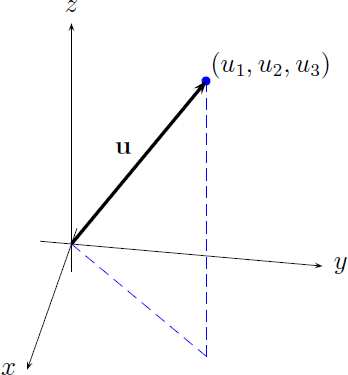
\includegraphics[scale=0.8]{images/vector-3d}
\caption{A vector in three-dimensional space.}
\label{fig:vectors_matrices:3D_vector}
\end{figure}

%% \begin{practice}
%% Let \emph{\vecu} be a three-dimensional vector and let $c$ be a
%% scalar. Show that $\vecvertl c \emph{\vecu}
%% \vecvertr = |c| \, \vecvertl \emph{\vecu}
%% \vecvertr$.
%% \end{practice}

%% \begin{practice}
%% \label{prac:triangle_inequality_three_dimensions}
%% Given two vectors $\emph{\vecu} = \langle 3, 5, 7 \rangle$ and
%% $\emph{\textbf{v}} = \langle -1, 2, 9 \rangle$, show that
%% $\vecvertl \emph{\vecu} + \emph{\textbf{v}}
%% \vecvertr \leq \vecvertl \emph{\vecu}
%% \vecvertr + \vecvertl \emph{\textbf{v}} \vecvertr$.
%% \end{practice}

\begin{figure}[!htpb]
\centering
%% \begin{pspicture}(-3,-1)(3,3)
%% \pstThreeDCoor[linecolor=black,xMin=-0.5,xMax=3,yMin=-0.5,yMax=3,zMin=-0.5,zMax=3]
%% \pstThreeDLine[linewidth=1.5pt,arrows=->](0,0,0)(2,0,0)
%% \pstThreeDLine[linewidth=1.5pt,arrows=->](0,0,0)(0,2,0)
%% \pstThreeDLine[linewidth=1.5pt,arrows=->](0,0,0)(0,0,2)
%% \uput[0](-2.7,-0.5){$(1,0,0)$}\uput[0](-1,-0.1){\veci}
%% \uput[0](1.2,-0.4){$(0,1,0)$}\uput[0](0.5,0){\vecj}
%% \uput[0](-0.1,1.8){$(0,0,1)$}\uput[0](0,1){\veck}
%% \end{pspicture}
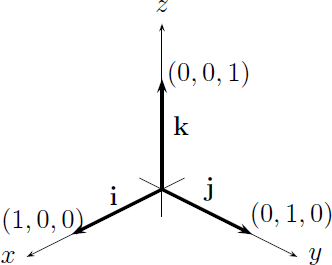
\includegraphics[scale=0.8]{images/unit-vectors-3d}
\caption{Unit vectors in three-dimensional space.}
\label{fig:vectors_matrices:unit_vectors_3D}
\end{figure}

If a nonzero vector $\vecu$ (in two- or three-dimensional space) is
multiplied by $1 / \vecvertl \vecu \vecvertr$, the result is a vector
of magnitude $1$. Vectors of magnitude $1$ are called
\emph{unit vectors}\index{unit vectors}. Thus the vector in
equation~(\ref{eq:vectors_matrices:two_dimensional_unit_vector}) is a
two-dimensional unit vector. Of particular interest in physics are the
\emph{standard unit vectors}\index{standard unit vectors}
\[
\veci = \langle 1, 0 \rangle
\qquad\text{and}\qquad
\vecj = \langle 0, 1 \rangle
\]
in the two-dimensional plane, and their three-dimensional
counterparts:
%
\begin{equation}
\label{eq:vectors_matrices:standard_unit_vectors_three_dimensions}
\veci = \langle 1, 0, 0 \rangle, \qquad
\vecj = \langle 0, 1, 0 \rangle, \qquad
\veck = \langle 0, 0, 1 \rangle.
\end{equation}
%
The three-dimensional standard unit vectors are shown in
Figure~\ref{fig:vectors_matrices:unit_vectors_3D}. These vectors play
a role similar to the number $1$, where every real number $a$ can be
expressed as $a = a \cdot 1$. So every three-dimensional~(respectively
two-dimensional) vector $\vecu = \langle u_1, u_2, u_3 \rangle$ can be
expressed in terms of the standard unit
vectors~(\ref{eq:vectors_matrices:standard_unit_vectors_three_dimensions})
as
\[
\vecu
=
\langle u_1, u_2, u_3 \rangle
=
\langle u_1, 0, 0 \rangle +
\langle 0, u_2, 0 \rangle + \langle 0, 0, u_3 \rangle
=
u_1 \veci + u_2 \vecj + u_3 \veck.
\]
For example, in the plane we have
$\langle 2, 3 \rangle = 2\veci + 3 \vecj$. In three-dimensional space
we have $\langle 5, -1, 7 \rangle = 5 \veci - \vecj + 7 \veck$, whose
magnitude is $5\sqrt{3}$ and so
\[
\frac{1}{5\sqrt{3}} \langle 5, -1, 7 \rangle
=
\frac{1}{\sqrt{3}}\veci
-
\frac{1}{5\sqrt{3}}\vecj
+
\frac{7}{5\sqrt{3}}\veck
\]
is a unit vector in the same direction as $\langle 5, -1, 7 \rangle$.


%%%%%%%%%%%%%%%%%%%%%%%%%%%%%%%%%%%%%%%%%%%%%%%%%%%%%%%%%%%%%%%%%%%%%%%%%%%

\section{The dot product}
\label{sec:dot_product}
\index{dot product}

Section~\ref{sec:scalars_vectors} discussed vectors and
showed how we can perform various arithmetic operations on them. In
particular, we have shown how a vector can be multiplied by a
scalar. We now consider the case of multiplying two vectors.

\begin{definition}
\label{def:vectors_matrices:vector_dot_product}
Let $\vecu = \langle u_1, u_2, u_3 \rangle$ and
$\vecv = \langle v_1, v_2, v_3 \rangle$ be
three-dimensional vectors. Then the vector
\emph{dot product}\index{dot product} of $\vecu$ and $\vecv$ is
defined as
\[
\vecu \cdot \vecv
=
u_1 v_1 + u_2 v_2 + u_3 v_3.
\]
\end{definition}

The vector dot product is also called the
scalar\index{scalar product} or inner\index{inner product}
product. Unlike scalar multiplication of a scalar $c$ and a vector
$\vecu$, which results in another vector $c\vecu$, the dot product of
two vectors $\vecu$ and $\vecv$ is a scalar. A similar definition
holds for two-dimensional vectors. Thus to find the dot product of two
vectors both of which are in two- or three-dimensional space, we
multiply the corresponding components and add up the results.

\begin{lstlisting}
sage: u = vector([3, 5, 7])
sage: v = vector([-2, 7, -9])
sage: # compute dot product from definition
sage: zip(u, v)
[(3, -2), (5, 7), (7, -9)]
sage: p = map(prod, zip(u, v)); p
[-6, 35, -63]
sage: sum(p)
-34
sage: # compute dot product using built-in functions
sage: u.dot_product(v)
-34
sage: u * v
-34
\end{lstlisting}

We can also find the dot product of two vectors in terms of the
angle\index{angle} between them. If $\theta$ is the angle between two
vectors $\vecu$ and $\vecv$ in two- or three-dimensional space, then
their dot product obeys the following geometric interpretation:
\index{dot product!geometric interpretation}
%
\begin{equation}
\label{eq:vectors_matrices:geometric_interpretation_dot_product}
\vecu \cdot \vecv
=
\begin{cases}
\vecvertl \vecu \vecvertr \,
\vecvertl \vecv \vecvertr \cos\theta
&\text{if $\vecu \neq \veczero$ and $\vecv \neq \veczero$}\\
0 & \text{if $\vecu = \veczero$ or $\vecv = \veczero$}.
\end{cases}
\end{equation}
%
Using the last equation, the angle between two nonzero vectors is
given by
%
\begin{equation}
\label{eq:vectors_matrices:angle_between_vectors}
\theta
=
\cos^{-1}
\left(
\frac {\vecu \cdot \vecv}
{\vecvertl \vecu \vecvertr \, \vecvertl \vecv \vecvertr}
\right).
\end{equation}

\begin{example}
Consider the vectors $\vecu = \langle 3, -1, 7 \rangle$
and $\vecv = \langle -2, 5, 8 \rangle$. Find the angle
between $\vecu$ and $\vecv$.
\end{example}

\begin{proof}[Solution]
To find the angle between two vectors, we use
equation~(\ref{eq:vectors_matrices:angle_between_vectors}). From
Definition~\ref{def:vectors_matrices:vector_dot_product}, the dot
product of $\vecu$ and $\vecv$ is
\[
\vecu \cdot \vecv
=
3(-2) + (-1)5 + 7(8)
=
45.
\]
Using
equation~(\ref{eq:vectors_matrices:magnitude_three_dimensional_vector}),
the magnitude of $\vecu$ is
$\vecvertl \vecu \vecvertr = \sqrt{9 + 1 + 49} = \sqrt{59}$ and that
of $\vecv$ is
$\vecvertl \vecv \vecvertr = \sqrt{4 + 25 + 64} = \sqrt{93}$.
Substitute the value of the dot product and the individual magnitudes
into equation~(\ref{eq:vectors_matrices:angle_between_vectors}) to get
\[
\theta
=
\cos^{-1} \left( \frac{45}{\sqrt{59 \cdot 93}} \right)
\]
which is the angle between $\vecu$ and $\vecv$. This angle can
be computed using Sage as follows:
%
\begin{lstlisting}
sage: u = vector([3, -1, 7]); v = vector([-2, 5, 8])
sage: numer = u * v
sage: denom = u.norm() * v.norm()
sage: arccos(numer / denom)
arccos(45/(sqrt(59)*sqrt(93)))
\end{lstlisting}
%
which is the same as what we have above.
\end{proof}

From plane geometry, we know that two lines are
perpendicular\index{perpendicular lines} if the angle $\theta$ between
them is $90^{\circ}$ or $\theta = \pi / 2$ radians. Now $\cos (\pi /
2) = 0$ and using
equation~(\ref{eq:vectors_matrices:geometric_interpretation_dot_product}),
we see that two non-zero vectors are perpendicular (also called
\emph{orthogonal})\index{vector!orthogonal}\index{orthogonal vectors}
if and only if their dot product is zero.


%%%%%%%%%%%%%%%%%%%%%%%%%%%%%%%%%%%%%%%%%%%%%%%%%%%%%%%%%%%%%%%%%%%%%%%%%%%

\section{Parallel and perpendicular vectors}
\index{parallel vectors}
\index{perpendicular vectors}

In section~\ref{sec:scalars_vectors}, we resolved a
two-dimensional vector into components that are parallel to the
axes. A similar technique can be used to resolve a three-dimensional
vector into components that are also parallel to the axes. We now
present another method for resolving a vector $\vecu$ into two
components $\vecu_{\vecpar}$ and $\vecu_{\vecper}$, which are parallel
and perpendicular to a given nonzero vector $\vecv$, respectively.

The left-hand side of
Figure~\ref{fig:vectors_matrices:_parallel_perpendicular_vectors} shows
the case where the angle $\theta$ between $\vecu$ and $\vecv$ is
$0 < \theta < \pi/2$; the right-hand side of the figure shows the case
where $\pi/2 < \theta < \pi$. We can think of
$\vecu_{\vecpar}$ as being the shadow\index{vector!shadow} of
$\vecu$ cast on the line in the direction of $\vecv$. Then the
magnitude of $\vecu_{\vecpar}$ is the length of the shadow. By
the triangle rule for vector difference~(see
Figure~\ref{fig:vectors_matrices:vector_difference_parallelogram_triangle}),
we have $\vecu_{\vecper} = \vecu - \vecu_{\vecpar}$. All it remains
now is to find an expression for $\vecu_{\vecpar}$ in terms of the
known vectors $\vecu$ and $\vecv$.

\begin{figure}[!htpb]
\centering
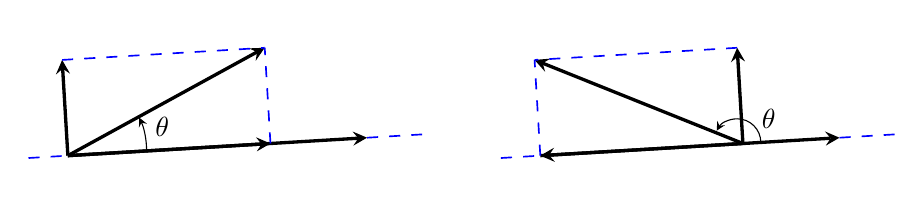
\begin{tikzpicture}
% left-hand side figure
\draw[->,>=stealth,very thick] (-0.5,0.03) -- (2,1.4) node[above]{$\vecu$};
\draw[->,>=stealth,very thick] (-0.5,0.03) -- (3.3,0.258) node[below]{$\vecv$};
\draw[->,>=stealth,very thick] (-0.5,0.03) -- node[below]{$\vecu_{\vecpar}$} (2.072937,0.184375);
\draw[->,>=stealth,very thick] (-0.5,0.03) -- node[left]{$\vecu_{\vecper}$} (-0.572937,1.245625);
\draw[color=blue,semithick,dash pattern=on 4pt off 4pt] (2.072937,0.184375) -- (2,1.4);
\draw[color=blue,semithick,dash pattern=on 4pt off 4pt] (-0.572937,1.245625) -- (2,1.4);
\draw[color=blue,semithick,dash pattern=on 4pt off 4pt] (-1,0) -- (-0.5,0.03);
\draw[color=blue,semithick,dash pattern=on 4pt off 4pt] (3.3,0.258) -- (4,0.3);
\draw[->,>=stealth] (0.5,0.089999) arc (0:25:1);
\node at (0.7,0.4) {$\theta$};
%
% right-hand side figure
\draw[->,>=stealth,very thick] (8.072937,0.184375) -- (5.427063,1.245625) node[above]{$\vecu$};
\draw[->,>=stealth,very thick] (5.5,0.03) -- (9.3,0.258) node[below]{$\vecv$};
\draw[->,>=stealth,very thick] (8.072937,0.184375) -- node[below]{$\vecu_{\vecpar}$} (5.5,0.03);
\draw[->,>=stealth,very thick] (8.072937,0.184375) -- (8,1.4) node[right]{$\vecu_{\vecper}$};
\draw[color=blue,semithick,dash pattern=on 4pt off 4pt] (8,1.4) -- (5.427063,1.245625);
\draw[color=blue,semithick,dash pattern=on 4pt off 4pt] (5.5,0.03) -- (5.427063,1.245625);
\draw[color=blue,semithick,dash pattern=on 4pt off 4pt] (9.3,0.258) -- (10,0.3);
\draw[color=blue,semithick,dash pattern=on 4pt off 4pt] (5,0) -- (5.5,0.03);
\draw[->,>=stealth] (8.3,0.198) arc (0:150:0.3);
\node at (8.4,0.5) {$\theta$};
\end{tikzpicture}
\caption{Resolving $\vecu$ into components parallel and
  perpendicular to $\vecv$. The angle between $\vecu$ and
  $\vecv$ is $0 < \theta < \pi/2$ (left) and $\pi/2 < \theta < \pi$
(right).}
\label{fig:vectors_matrices:_parallel_perpendicular_vectors}
\end{figure}

Since $\vecu_{\vecpar}$ and $\vecv$ are parallel, then one
is a scalar multiple of the other, that is
%
\begin{equation}
\label{eq:vectors_matrices:u_par_parallel_v}
\vecu_{\vecpar}
=
c\vecv
\end{equation}
%
for some scalar $c \neq 0$. Using the parallelogram
rule\index{parallelogram rule} for vector addition, we have
$\vecu = \vecu_{\vecpar} + \vecu_{\vecper}$. Then the dot product of
$\vecu$ and $\vecv$ is
%
\begin{equation}
\label{eq:vectors_matrices:u_per_orthogonal_v}
\begin{aligned}
\vecu \cdot \vecv
&=
(\vecu_{\vecpar} + \vecu_{\vecper}) \cdot \vecv \\
&=
\vecu_{\vecpar} \cdot \vecv +
\vecu_{\vecper} \cdot \vecv.
\end{aligned}
\end{equation}
%
By definition, $\vecu_{\vecper}$ is orthogonal to $\vecv$,
hence their dot product is zero. Using this fact and
substituting~(\ref{eq:vectors_matrices:u_par_parallel_v})
into~(\ref{eq:vectors_matrices:u_per_orthogonal_v}), we see that
equation~(\ref{eq:vectors_matrices:u_per_orthogonal_v}) simplifies to
%
\begin{align*}
\vecu \cdot \vecv
&=
\vecu_{\vecpar} \cdot \vecv \\
&=
(c \vecv) \cdot \vecv \\
&=
c (\vecv \cdot \vecv).
\end{align*}
%
Solving the last equation for $c$, we have $c = \frac {\vecu \cdot
\vecv} {\vecv \cdot \vecv}$. Substitute this into
equation~(\ref{eq:vectors_matrices:u_par_parallel_v}) results in
%
\begin{align}
\vecu_{\vecpar}
&=
\frac {\vecu \cdot \vecv} {\vecv \cdot \vecv}
\vecv %
\label{eq:vectors_matrices:u_par_vector_projection} \\[4pt]
\vecu_{\vecper}
&=
\vecu - \vecu_{\vecpar}. %
\label{eq:vectors_matrices:u_per_scalar_projection}
\end{align}
%
The upshot is that given two nonzero vectors $\vecu$ and
$\vecv$, equations~(\ref{eq:vectors_matrices:u_par_vector_projection})
and~(\ref{eq:vectors_matrices:u_per_scalar_projection}) allow us to
resolve $\vecu$ into two component vectors $\vecu_{\vecpar}$ and
$\vecu_{\vecper}$ that are, respectively,
parallel\index{parallel vectors} and
orthogonal\index{orthogonal vectors} to $\vecv$.

\begin{example}
\index{vectors!projection}
Let $\vecu = \langle 3, 4, -5 \rangle$ and
$\vecv = \langle -7, 8, 9 \rangle$. Find the projection of $\vecu$
onto $\vecv$, and a vector that is orthogonal to $\vecv$.
\end{example}

\begin{proof}[Solution]
To compute the projection of $\vecu$ onto $\vecv$, we use
equation~(\ref{eq:vectors_matrices:u_par_vector_projection}). So
$\vecu \cdot \vecv = 3(-7) + 4(8) - 5(9) = -34$ and
$\vecv \cdot \vecv = (-7)^2 + 8^2 + 9^2 = 194$. Then
\[
\vecu_{\vecpar}
=
-\frac{34}{194} \langle -7, 8, 9 \rangle
=
\left\langle
\frac{119}{97},\, -\frac{136}{97},\, -\frac{153}{97}
\right\rangle.
\]
Next we use
equation~(\ref{eq:vectors_matrices:u_per_scalar_projection}) to find a
vector that is parallel to $\vecv$. Then
\[
\vecu_{\vecper}
=
\langle 3, 4, -5 \rangle -
\left\langle
\frac{119}{97},\, -\frac{136}{97},\, -\frac{153}{97}
\right\rangle
=
\left\langle
\frac{172}{97},\, \frac{524}{97},\, -\frac{332}{97}
\right\rangle
\]
as required. Using Sage, we get
%
\begin{lstlisting}
sage: u = vector([3, 4, -5])
sage: v = vector([-7, 8, 9])
sage: u_par = ((u*v) / (v*v)) * v; u_par
(119/97, -136/97, -153/97)
sage: u_per = u - u_par; u_per
(172/97, 524/97, -332/97)
\end{lstlisting}
%
which agrees with our calculation above.
\end{proof}


%%%%%%%%%%%%%%%%%%%%%%%%%%%%%%%%%%%%%%%%%%%%%%%%%%%%%%%%%%%%%%%%%%%%%%%%%%%

\section{Matrices and determinants}
\index{determinant}
\index{matrix}

A $2 \times 2$ \emph{matrix}\index{matrix} is an array of numbers
organized as follows:
%
\begin{equation}
\label{eq:vectors_matrices:2_by_2_matrix}
\begin{bmatrix}
a & b \\
c & d
\end{bmatrix}
\end{equation}
%
which has $2$ rows and $2$ columns. Similarly, a $3 \times 3$ matrix
is an array with $3$ rows and $3$ columns:
%
\begin{equation}
\label{eq:vectors_matrices:3_by_3_matrix}
\begin{bmatrix}
a_1 & a_2 & a_3 \\
b_1 & b_2 & b_3 \\
c_1 & c_2 & c_3
\end{bmatrix}.
\end{equation}
%
Matrices of higher dimensions are similarly defined. Each number in a
matrix is called its \emph{entry}\index{entry}.

Just as we can manipulate vectors using the familiar rules of
arithmetic, we can also work with matrices using many of those same
rules. To understand how we can add, subtract, and multiply matrices,
let $s$ be a scalar and let $A,B,C,D$ be matrices defined as follows:
%
\begin{align*}
A
=
\begin{bmatrix}
a_{11} & a_{12} \\
a_{21} & a_{22}
\end{bmatrix},
&\qquad
B
=
\begin{bmatrix}
b_{11} & b_{12} \\
b_{21} & b_{22}
\end{bmatrix}, \\[4pt]
%
C
=
\begin{bmatrix}
c_{11} & c_{12} & c_{13} \\
c_{21} & c_{22} & c_{23} \\
c_{31} & c_{32} & c_{33}
\end{bmatrix},
&\qquad
D
=
\begin{bmatrix}
d_{11} & d_{12} & d_{13} \\
d_{21} & d_{22} & d_{23} \\
d_{31} & d_{32} & d_{33}
\end{bmatrix}.
\end{align*}
%
Only matrices of the same dimensions can be added and
subtracted. Since $A$ and $B$ are both $2 \times 2$ matrices, we can
add and subtract them according to the rules
%
\begin{align*}
A + B
&=
\begin{bmatrix}
a_{11} & a_{12} \\
a_{21} & a_{22}
\end{bmatrix}
+
\begin{bmatrix}
b_{11} & b_{12} \\
b_{21} & b_{22}
\end{bmatrix}
=
\begin{bmatrix}
a_{11} + b_{11} & a_{12} + b_{12} \\
a_{21} + b_{21} & a_{22} + b_{22}
\end{bmatrix}, \\[4pt]
%
A - B
&=
\begin{bmatrix}
a_{11} & a_{12} \\
a_{21} & a_{22}
\end{bmatrix}
-
\begin{bmatrix}
b_{11} & b_{12} \\
b_{21} & b_{22}
\end{bmatrix}
=
\begin{bmatrix}
a_{11} - b_{11} & a_{12} - b_{12} \\
a_{21} - b_{21} & a_{22} - b_{22}
\end{bmatrix}.
\end{align*}
%
That is, to add or subtract two matrices of the same dimensions, we
add or subtract the corresponding entries. We can add or subtract the
matrices $C$ and $D$ using this principle.

\begin{lstlisting}
sage: # general rules for adding and subtracting matrices
sage: var("a_11, a_12, a_21, a_22");
sage: var("b_11, b_12, b_21, b_22");
sage: A = matrix([[a_11, a_12], [a_21, a_22]]); A
[a_11 a_12]
[a_21 a_22]
sage: B = matrix([[b_11, b_12], [b_21, b_22]]); B
[b_11 b_12]
[b_21 b_22]
sage: A + B
[a_11 + b_11 a_12 + b_12]
[a_21 + b_21 a_22 + b_22]
sage: A - B
[a_11 - b_11 a_12 - b_12]
[a_21 - b_21 a_22 - b_22]
sage: # some examples of matrix addition and subtraction
sage: A = matrix([[1,2], [3,4]]); A
[1 2]
[3 4]
sage: B = matrix([[2,3], [5,7]]); B
[2 3]
[5 7]
sage: A + B
[ 3  5]
[ 8 11]
sage: A - B
[-1 -1]
[-2 -3]
\end{lstlisting}

To multiply a scalar by a matrix, we multiply the scalar by each
entry. That is,
\[
sA
=
s
\begin{bmatrix}
a_{11} & a_{12} \\
a_{21} & a_{22}
\end{bmatrix}
=
\begin{bmatrix}
sa_{11} & sa_{12} \\
sa_{21} & sa_{22}
\end{bmatrix}
\]
and similarly for $3 \times 3$ matrices.

\begin{lstlisting}
sage: var("a_11, a_12, a_21, a_22, s");
sage: A = matrix([[a_11, a_12], [a_21, a_22]]); A
[a_11 a_12]
[a_21 a_22]
sage: s*A
[a_11*s a_12*s]
[a_21*s a_22*s]
sage: A = matrix([[1,2], [3,4]]); A
[1 2]
[3 4]
sage: 3*A
[ 3  6]
[ 9 12]
\end{lstlisting}

But how are we to multiply two matrices of the same dimensions? The
rule for multiplying two $2 \times 2$ matrices is
\[
AB
=
\begin{bmatrix}
a_{11} & a_{12} \\
a_{21} & a_{22}
\end{bmatrix}
%
\begin{bmatrix}
b_{11} & b_{12} \\
b_{21} & b_{22}
\end{bmatrix}
=
\begin{bmatrix}
a_{11} b_{11} + a_{12} b_{21} & a_{11} b_{12} + a_{12} b_{22} \\
a_{21} b_{11} + a_{22} b_{21} & a_{21} b_{12} + a_{22} b_{22}
\end{bmatrix}.
\]
To multiply two $3 \times 3$ matrices, we use
%
\begin{align*}
CD
&=
\begin{bmatrix}
c_{11} & c_{12} & c_{13} \\
c_{21} & c_{22} & c_{23} \\
c_{31} & c_{32} & c_{33}
\end{bmatrix}
%
\begin{bmatrix}
d_{11} & d_{12} & d_{13} \\
d_{21} & d_{22} & d_{23} \\
d_{31} & d_{32} & d_{33}
\end{bmatrix} \\[4pt]
&=
\begin{bmatrix}
c_{11} d_{11} + c_{12} d_{21} + c_{13} d_{31} &
c_{11} d_{12} + c_{12} d_{22} + c_{13} d_{32} &
c_{11} d_{13} + c_{12} d_{23} + c_{13} d_{33} \\
%
c_{21} d_{11} + c_{22} d_{21} + c_{23} d_{31} &
c_{21} d_{12} + c_{22} d_{22} + c_{23} d_{32} &
c_{21} d_{13} + c_{22} d_{23} + c_{23} d_{33} \\
c_{31} d_{11} + c_{32} d_{21} + c_{33} d_{31} &
c_{31} d_{12} + c_{32} d_{22} + c_{33} d_{32} &
c_{31} d_{13} + c_{32} d_{23} + c_{33} d_{33}
\end{bmatrix}.
\end{align*}

\begin{lstlisting}
sage: var("a_11, a_12, a_21, a_22");
sage: var("b_11, b_12, b_21, b_22");
sage: A = matrix([[a_11, a_12], [a_21, a_22]])
sage: B = matrix([[b_11, b_12], [b_21, b_22]])
sage: A * B
[a_11*b_11 + a_12*b_21 a_11*b_12 + a_12*b_22]
[a_21*b_11 + a_22*b_21 a_21*b_12 + a_22*b_22]
sage: A = matrix([[1,2], [3,4]])
sage: B = matrix([[3,5], [7,9]])
sage: A * B
[17 23]
[37 51]
sage: C = matrix([[1,2,3], [4,5,6], [7,8,9]]); C
[1 2 3]
[4 5 6]
[7 8 9]
sage: D = matrix([[-1,1,3], [4,0,6], [7,2,4]]); D
[-1  1  3]
[ 4  0  6]
[ 7  2  4]
sage: C * D
[ 28   7  27]
[ 58  16  66]
[ 88  25 105]
\end{lstlisting}

As far as matrices go, they are a convenient notation for organizing a
bunch of numbers. Things get interesting when we take the
\emph{determinant}\index{determinant} of a $2 \times 2$ or
$3 \times 3$ matrix. The determinant of the $2 \times 2$
matrix~(\ref{eq:vectors_matrices:2_by_2_matrix}) is defined as
\[
\begin{vmatrix}
a & b \\
c & d
\end{vmatrix}
=
ad - bc
\]
which, like the dot product, is a scalar. For example,
\[
\begin{vmatrix}
-2 & 7 \\
9  & 1
\end{vmatrix}
=
-2(1) - 7(9)
=
-65.
\]

\begin{lstlisting}
sage: var("a, b, c, d");
sage: A = matrix([[a,b], [c,d]]); A
[a b]
[c d]
sage: A.det()
a*d - b*c
sage: A = matrix([[-2,7], [9,1]]); A
[-2  7]
[ 9  1]
sage: A.det()
-65
\end{lstlisting}

The formula for $2 \times 2$ determinants is short and
straightforward. However, the same cannot be said for $3 \times 3$
determinants. The determinant of the $3 \times 3$
matrix~(\ref{eq:vectors_matrices:3_by_3_matrix}) is defined in terms
of $2 \times 2$
determinants as follows:
%
\begin{equation}
\label{eq:vectors_matrices:3_by_3_determinant}
\begin{vmatrix}
a_1 & a_2 & a_3 \\
b_1 & b_2 & b_3 \\
c_1 & c_2 & c_3
\end{vmatrix}
=
a_1
\begin{vmatrix}
b_2 & b_3 \\
c_2 & c_3
\end{vmatrix}
-
a_2
\begin{vmatrix}
b_1 & b_3 \\
c_1 & c_3
\end{vmatrix}
+
a_3
\begin{vmatrix}
b_1 & b_2 \\
c_1 & c_2
\end{vmatrix}.
\end{equation}
%
For example,
%
\begin{align*}
\begin{vmatrix}
2  & -1 & 5 \\
7  & 6  & 9 \\
-1 & 3  & 4
\end{vmatrix}
&=
2
\begin{vmatrix}
6 & 9 \\
3 & 4
\end{vmatrix}
-
(-1)
\begin{vmatrix}
7  & 9 \\
-1 & 4
\end{vmatrix}
+
5
\begin{vmatrix}
7  & 6 \\
-1 & 3
\end{vmatrix} \\
&= 2 \big( 6(4) - 9(3) \big)
 - (-1) \big( 7(4) - 9(-1) \big)
 + 5 \big( 7(3) - 6(-1) \big) \\
&=
-6 - (-37) + 135 \\
&=
166.
\end{align*}

\begin{lstlisting}
sage: var("a_1, a_2, a_3, b_1, b_2, b_3, c_1, c_2, c_3");
sage: B = matrix([[a_1,a_2,a_3], [b_1,b_2,b_3], [c_1,c_2,c_3]]); B
[a_1 a_2 a_3]
[b_1 b_2 b_3]
[c_1 c_2 c_3]
sage: B.det()
(b_2*c_3 - b_3*c_2)*a_1 - (a_2*c_3 - a_3*c_2)*b_1 + (a_2*b_3 - a_3*b_2)*c_1
sage: B = matrix([[2,-1,5], [7,6,9], [-1,3,4]]); B
[ 2 -1  5]
[ 7  6  9]
[-1  3  4]
sage: B.det()
166
\end{lstlisting}


%%%%%%%%%%%%%%%%%%%%%%%%%%%%%%%%%%%%%%%%%%%%%%%%%%%%%%%%%%%%%%%%%%%%%%%%%%%

\section{The cross product}
\index{cross product}

We have seen that scalar multiplication produces a vector, while the
dot product results in a scalar. This section presents another
operation on vectors, called the cross product, that produces
a vector as a result. Unlike scalar multiplication and dot product,
the cross product is not defined for two-dimensional vectors.

Let $\vecu = \langle u_1, u_2, u_3 \rangle$ and
$\vecv = \langle v_1, v_2, v_3 \rangle$ be three-dimensional vectors,
and let $\veci, \vecj, \veck$ be the standard unit vectors in
three-dimensional space. Then the
\emph{cross product}\index{cross product} of $\vecu$ and $\vecv$ is
defined as the vector
\[
\vecu \times \vecv
=
\begin{vmatrix}
u_2 & u_3 \\
v_2 & v_3
\end{vmatrix}
\veci
-
\begin{vmatrix}
u_1 & u_3 \\
v_1 & v_3
\end{vmatrix}
\vecj
+
\begin{vmatrix}
u_1 & u_2 \\
v_1 & v_2
\end{vmatrix}
\veck.
\]
Here is a mnemonic trick to remember the definition of the cross
product:
%
\begin{equation}
\label{eq:vectors_matrices:mnemonic_cross_product}
\vecu \times \vecv
=
\begin{vmatrix}
\veci & \vecj & \veck \\
u_1 & u_2 & u_3 \\
v_1 & v_2 & v_3
\end{vmatrix}.
\end{equation}
%
Expand this determinant using the
formula~(\ref{eq:vectors_matrices:3_by_3_determinant}). The entries of
matrices we work with should be numbers, not vectors. Strictly
speaking, it does not make sense to have the standard unit vectors
$\veci$, $\vecj$, and $\veck$ as matrix entries. We stress that
equation~(\ref{eq:vectors_matrices:mnemonic_cross_product}) is just a
trick to remember the definition of the cross product.

\begin{lstlisting}
sage: var("u_1, u_2, u_3");
sage: var("v_1, v_2, v_3");
sage: u = vector([u_1, u_2, u_3])
sage: v = vector([v_1, v_2, v_3])
sage: u.cross_product(v)
(u_2*v_3 - u_3*v_2, -u_1*v_3 + u_3*v_1, u_1*v_2 - u_2*v_1)
\end{lstlisting}

Like the dot product, the cross product also shares a number of
arithmetic properties of ordinary numbers. Let $\vecu$, $\vecv$, and
$\vecw$ be three-dimensional vectors and suppose $c$ is a scalar. Then
the cross product has the following properties:
%
\begin{enumerate}
\item Anticommutative\index{anticommutative}:
  $\vecu \times \vecv = - \vecv \times \vecu$.

\item Distributive\index{distributive}:
  $\vecu \times (\vecv + \vecw)
  =
  \vecu \times \vecv + \vecu \times \vecw$.

\item Distributive:
  $(\vecu + \vecv) \times \vecw
  =
  \vecu \times \vecw + \vecv \times \vecw$.

\item Associative scalar multiplication\index{scalar multiplication}:
  $c (\vecu \times \vecv)
  =
  (c\vecu) \times \vecv
  = \vecu \times (c\vecv)$.

\item Zero element\index{zero element}:
  $\veczero \times \vecu
  =
  \veczero
  =
  \vecu \times \veczero$.

\item Self-inverse\index{self-inverse}: $\vecu \times \vecu = \veczero$.
\end{enumerate}

If $\vecu = \langle u_1, u_2, u_3 \rangle$ and
$\vecv = \langle v_1, v_2, v_3 \rangle$ are nonzero, then by the
definition of the cross product we have
%
\begin{align*}
\vecu \times \vecv
&=
\begin{vmatrix}
u_2 & u_3 \\
v_2 & v_3
\end{vmatrix}
\veci
-
\begin{vmatrix}
u_1 & u_3 \\
v_1 & v_3
\end{vmatrix}
\vecj
+
\begin{vmatrix}
u_1 & u_2 \\
v_1 & v_2
\end{vmatrix}
\veck \\
&=
\left\langle
u_2 v_3 - u_3 v_2,\; u_3 v_1 - u_1 v_3,\; u_1 v_2 - u_2 v_1
\right\rangle.
\end{align*}
%
The dot product of $\vecu$ and the last equation is
%
\begin{align*}
\vecu \cdot (\vecu \times \vecv)
&=
u_1 ( u_2 v_3 - u_3 v_2 ) +
u_2 ( u_3 v_1 - u_1 v_3 ) +
u_3 ( u_1 v_2 - u_2 v_1 ) \\
&=
0.
\end{align*}
%
Again by direct computation, we see that the dot product of $\vecv$
and $\vecu \times \vecv$ is
%
\begin{align*}
\vecv \cdot (\vecu \times \vecv)
&=
v_1 ( u_2 v_3 - u_3 v_2 ) +
v_2 ( u_3 v_1 - u_1 v_3 ) +
v_3 ( u_1 v_2 - u_2 v_1 ) \\
&=
0.
\end{align*}
%
From section~\ref{sec:dot_product}, we know that two nonzero vectors
are perpendicular\index{perpendicular vectors} if and only if their
dot product is zero. The last two equations show that $\vecu$ and
$\vecv$ are both perpendicular to $\vecu \times \vecv$. In other
words, we have proved the following result.

\begin{theorem}
\label{thm:vectors_matrices:u_v_parallel_u_dot_v}
If $\vecu$ and $\vecv$ are nonzero vectors in three-dimensional space,
then both of them are orthogonal to $\vecu \times \vecv$. That is
\[
\vecu \cdot (\vecu \times \vecv)
=
0
=
\vecv \cdot (\vecu \times \vecv).
\]
\end{theorem}

Similarly, we can also prove
Theorem~\ref{thm:vectors_matrices:more_properties_cross_product} using
direct calculation. Here is a proof using Sage:
%
\begin{lstlisting}
sage: var("u_1, u_2, u_3");
sage: var("v_1, v_2, v_3");
sage: var("w_1, w_2, w_3");
sage: # prove perpendicularity property
sage: u = vector([u_1, u_2, u_3])
sage: v = vector([v_1, v_2, v_3])
sage: w = vector([w_1, w_2, w_3])
sage: u * (u.cross_product(v))
(u_2*v_3 - u_3*v_2)*u_1 - (u_1*v_3 - u_3*v_1)*u_2 + (u_1*v_2 - u_2*v_1)*u_3
sage: expand(u * (u.cross_product(v)))
0
sage: v * (u.cross_product(v))
(u_2*v_3 - u_3*v_2)*v_1 - (u_1*v_3 - u_3*v_1)*v_2 + (u_1*v_2 - u_2*v_1)*v_3
sage: expand(v * (u.cross_product(v)))
0
sage: # prove matrix property
sage: u.cross_product(v.cross_product(w)) == (u*w)*v - (u*v)*w
True
sage: m = matrix([list(u), list(v), list(w)]); m
[u_1 u_2 u_3]
[v_1 v_2 v_3]
[w_1 w_2 w_3]
sage: bool(u*(v.cross_product(w)) == m.det())
True
\end{lstlisting}

\begin{theorem}
\label{thm:vectors_matrices:more_properties_cross_product}
If $\vecu$ and $\vecv$ are nonzero vectors in three-dimensional space,
then we have
%
\begin{enumerate}
\item
  $\vecu \times (\vecv \times \vecw)
  =
  (\vecu \cdot \vecw) \vecv - (\vecu \cdot \vecv) \vecw$.

\item
  $\vecu \cdot (\vecv \times \vecw)
  =
  \begin{vmatrix}
    u_1 & u_2 & u_3 \\
    v_1 & v_2 & v_3 \\
    w_1 & w_2 & w_3
  \end{vmatrix}$.
\end{enumerate}
\end{theorem}


%%%%%%%%%%%%%%%%%%%%%%%%%%%%%%%%%%%%%%%%%%%%%%%%%%%%%%%%%%%%%%%%%%%%%%%%%%%

\section*{Problems}
\addcontentsline{toc}{section}{Problems}

\begin{enumerate}
\item Consider the vectors in
  Figure~\ref{fig:vectors_matrices:verify_vectors_u_v}. Find the
  component forms of those vectors. Use the component forms to show
  that the vectors are equivalent.

\item \label{prob:vectors_matrices:field_laws_for_vectors}
  Let $\vecu$, $\vecv$ and $\vecw$ be vectors, all of which are either
  two- or three-dimensional. Suppose $c$ and $d$ are scalars. Show
  that these vectors have the following properties.
  \begin{enumerate}
  \item Commutative addition: $\vecu + \vecv = \vecv + \vecu$.

  \item Associative addition:
    $(\vecu + \vecv) + \vecw = \vecu + (\vecv + \vecw)$.

  \item Additive identity:
    $\vecu + \veczero = \vecu = \veczero + \vecu$.

  \item Additive inverse:
    $\vecu + (-\vecu) = \veczero = (-\vecu) + \vecu$.

  \item Associative scalar multiplication:
    $c (d \vecu) = (cd) \vecu$.

  \item Distributive over scalar addition:
    $(c + d) \vecu = c\vecu + d\vecu$.

  \item Distributive over vector addition:
    $c (\vecu + \vecv) = c\vecu + c\vecv$.

  \item Multiplicative identity:
    $1 (\vecu) = \vecu = (\vecu) 1$.

  \item Multiplication by zero:
    $0 (\vecu) = \veczero = (\vecu) 0$.
  \end{enumerate}

\item Show that $
  \vecvertl c\vecu \vecvertr
  =
  \left\arrowvert
  c\right\arrowvert \, \vecvertl \vecu
  \vecvertr$. Is this true for both two- and three-dimensional
  vectors?

\item Let $\vecu = \langle 3, 4 \rangle$ and
  $\vecv = \langle 9, 11 \rangle$. Show that $
  \vecvertl \vecu + \vecv\vecvertr
  \leq
  \vecvertl \vecu \vecvertr
  +
  \vecvertl \vecv \vecvertr$. Verify this inequality for
  three-dimensional vectors.

\item Let $(2, 17)$ and $(1/5,\, 8)$ be two points on a line
  $\ell$. Find a linear equation describing $\ell$. Express $\ell$ in
  vector form.

\item Let $\vecu = \langle 3, 7 \rangle$ and
  $\vecv = \langle -2, 5, 8 \rangle$. Express $\vecu$ and $\vecv$ in
  terms of standard unit vectors of the respective
  dimensions. Normalize $\vecu$ and $\vecv$ and express your results
  in terms of the appropriate standard unit vectors.

\item Consider the parallelogram in
  Figure~\ref{fig:vectors_matrices:diagonals_bisect}. The directed
  line segment from $O$ to $P$, for example, can be represented as the
  vector $\vecp = \overrightarrow{OP}$. Any other directed line
  segments in the figure can be similarly represented. Show that the
  diagonal lines of the parallelogram\index{parallelogram} bisect each
  other.
%
\begin{figure}[!htpb]
\centering
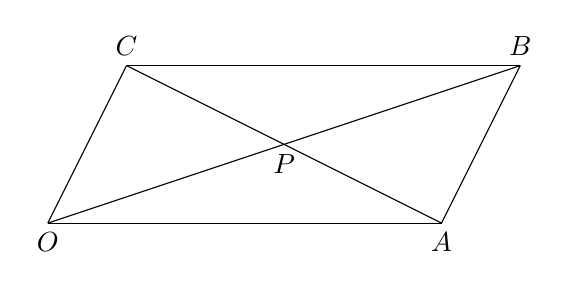
\begin{tikzpicture}
% parallelogram
\draw (0,0) node[below]{$O$} -- (5,0) node[below]{$A$};
\draw (0,0) -- (1,2) node[above]{$C$};
\draw (1,2) -- (6,2);
\draw (5,0) -- (6,2) node[above]{$B$};
% diagonals of the parallelogram
\draw (0,0) -- (6,2);
\draw (5,0) -- node[below]{$P$} (1,2);
\end{tikzpicture}
\caption{The diagonals bisect each other.}
\label{fig:vectors_matrices:diagonals_bisect}
\end{figure}

\item Given the vectors $\vecu = \langle u_1, u_2 \rangle$ and
  $\textbf{v} = \langle v_1, v_2, v_3 \rangle$, we can represent them
  in matrix notation as\index{vectors!matrix representation}\index{matrix}
  \[
  \vecu = \begin{bmatrix} u_1 \\ u_2 \end{bmatrix}
  \qquad\text{and}\qquad
  \textbf{v} = \begin{bmatrix} v_1 \\ v_2 \\ v_3 \end{bmatrix}.
  \]
  Express the standard unit vectors in matrix notation. Consider the
  vector operations in
  problem~\ref{prob:vectors_matrices:field_laws_for_vectors}. How
  would these be performed using matrix notation for vectors?

\item Consider
  Figure~\ref{fig:vectors_matrices:which_two_points_closest}, which
  shows the coordinates of your home~(point $H$), and that of your
  friends Emily~(point $E$) and David~(point $D$). Which of your two
  friends are closest to you? Who are closest to each other?
%
\begin{figure}
\centering
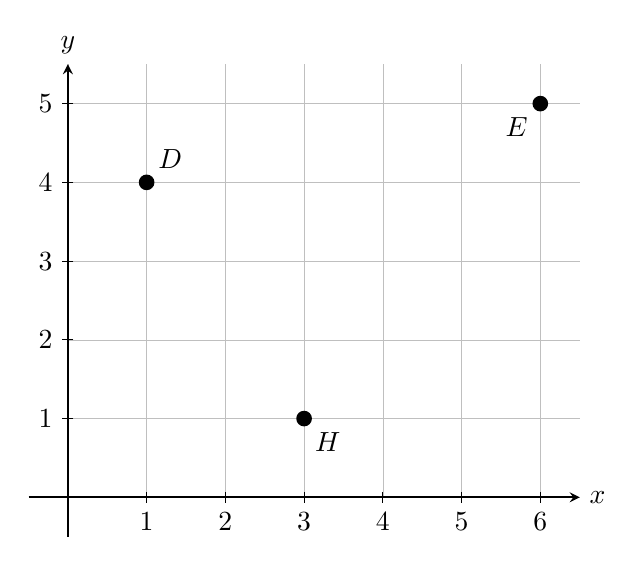
\begin{tikzpicture}
[linedecorate/.style={->,>=stealth,semithick},%
 nodedecorate/.style={fill=black,circle,inner sep=2pt}]
% grids for the plane
\draw[step=1cm,lightgray,very thin] (0,0) grid (6.5,5.5);
% the rectangular axes
\draw[linedecorate] (-0.5,0) -- (6.5,0) node[right]{$x$};
\draw[linedecorate] (0,-0.5) -- (0,5.5) node[above]{$y$};
% ticks on horizontal axis
\foreach \x in {1,2,...,6}
  \draw (\x cm,2pt) -- (\x cm,-2pt) node[anchor=north] {$\x$};
% ticks on vertical axis
\foreach \y in {1,2,...,5}
  \draw (2pt,\y cm) -- (-2pt,\y cm) node[anchor=east] {$\y$};
% points
\node[nodedecorate] at (1,4) {}; \node at (1.3,4.3) {$D$};
\node[nodedecorate] at (6,5) {}; \node at (5.7,4.7) {$E$};
\node[nodedecorate] at (3,1) {}; \node at (3.3,0.7) {$H$};
\end{tikzpicture}
\caption{Which two points are closest?}
\label{fig:vectors_matrices:which_two_points_closest}
\end{figure}

\item Let $\vecu = \langle 3, 5, 7 \rangle$ and
  $\vecv = \langle -2, 7, -9 \rangle$. Is it true that
  $\vecu \cdot \vecv = \vecv \cdot \vecu$ for these two particular
  vectors? Now let $\vecu$ and $\vecv$ be vectors, both of which are
  either two- or three-dimensional. Show that
  \[
  \vecu \cdot \vecv
  =
  \vecv \cdot \vecu
  \]
  and hence it does not matter in which order we perform the dot
  product.

\item Consider the vectors $\vecu$ and $\vecv$ in
  Figure~\ref{fig:vectors_matrices:maximum_minimum_dot_product}. Suppose
  the position of $\vecu$ is fixed and that it has magnitude
  $4$. Furthermore, $\vecv$ has magnitude $9$ and it is free to rotate
  from zero to $135$ degrees starting from the $x$-axis. Find the
  maximum and minimum values of $\vecu \cdot \vecv$. Which positions
  of $\vecu$ and $\vecv$ give rise to these maximum and minimum values?
%
\begin{figure}[!htpb]
\centering
\begin{tikzpicture}
% the rectangular axes
\draw[->,>=stealth,semithick] (-4,0) -- (4,0) node[right]{$x$};
\draw[->,>=stealth,semithick] (0,-0.2) -- (0,3.5) node[above]{$y$};
% vectors
\draw[->,>=stealth,very thick] (0,0) -- node[above left]{$\vecu$} (2.5,1.2);
\draw[->,>=stealth,very thick] (0,0) -- node[above right]{$\vecv$} (-3.5,2.8);
% angles between vectors and x-axis
\draw[->,>=stealth] (1,0) arc (0:25:1);
\node at (1.4,0.3) {$30^{\circ}$};
\draw[->,>=stealth] (-0.8,0.65) arc (135:176:1);
\node at (-1.3,0.45) {$45^{\circ}$};
\end{tikzpicture}
\caption{What are the maximum and minimum values of $\vecu \cdot \vecv$?}
\label{fig:vectors_matrices:maximum_minimum_dot_product}
\end{figure}

\item We can extend the results of
  problem~\ref{prob:vectors_matrices:field_laws_for_vectors} to
  include a number of arithmetic properties of the dot
  product. Let $\vecu$, $\vecv$, and $\vecw$ be vectors and let $c$ be
  a scalar. Show that the following properties hold for vectors in two
  and three dimensions.
  \begin{enumerate}
  \item $\vecu \cdot \vecu = \vecvertl \vecu \vecvertr^2$.

  \item Commutativity: $\vecu \cdot \vecv = \vecv \cdot \vecu$.

  \item Distributive property:
    $\vecu \cdot (\vecv + \vecw)
    =
    \vecu \cdot \vecv + \vecu \cdot \vecw$.

  \item Associative with respect to scalar multiplication:
    $c (\vecu \cdot \vecv)
    =
    (c \vecu) \cdot \vecv
    =
    \vecu \cdot (c \vecv)$.

  \item Zero vector:
    $\veczero \cdot \vecu = 0 = \vecu \cdot \veczero$.
  \end{enumerate}

\item Recall the standard unit vectors
  $\veci = \langle 1, 0 \rangle$ and $\vecj = \langle 0, 1 \rangle$ in
  the plane, and their three-dimensional counterparts
  $\veci = \langle 1, 0, 0 \rangle$,
  $\vecj = \langle 0, 1, 0 \rangle$, and
  $\veck = \langle 0, 0, 1 \rangle$. Show that the two-dimensional
  standard unit vectors are orthogonal. Show that any pair of
  three-dimensional standard unit vectors are orthogonal.

\item Let $\vecu$ be a vector whose tail is $(-1, 2, 4)$ and whose
  head is $(7, -1, 0)$. Let $\vecv$ be the vector
  $\langle 0, 4, 8 \rangle$. Resolve $\vecu$ into component vectors
  that are parallel and perpendicular to $\vecv$.

\item Let $\vecu$ and $\vecv$ be nonzero orthogonal vectors. What is
  the projection of $\vecu$ onto $\vecv$? What is the component vector
  of $\vecu$ that is perpendicular to $\vecv$?

\item Now suppose that $\vecu$ and $\vecv$ are nonzero parallel
  vectors. What is the projection of $\vecu$ onto $\vecv$? What is the
  component vector of $\vecu$ that is perpendicular to $\vecv$?

\item Let $A$ and $B$ be matrices, both of which are either $2 \times 2$
  or $3 \times 3$. In general, is the matrix product $AB$ equal to $BA$?

\item Consider the vectors $\vecu = \langle 4, 2, 1 \rangle$
  and $\vecv = \langle 6, 9, -7 \rangle$. Find the cross products
  $\vecu \times \vecv$ and $\vecv \times \vecu$.

\item Let $\vecu$ and $\vecv$ be three-dimensional vectors. Is it true
  that in general we have $\vecu \times \vecv = \vecv \times \vecu$?
  Explain your answer.

\item Let $\vecu$ and $\vecv$ be three-dimensional vectors. Show
  that
  \[
  \vecvertl \vecu \times \vecv \vecvertr^2
  =
  \vecvertl \vecu \vecvertr^2 \,
  \vecvertl \vecv \vecvertr^2
  -
  (\vecu \cdot \vecv)^2.
  \]
  This is known as Lagrange's identity\index{Lagrange's identity},
  named after Joseph-Louis
  Lagrange~(1736--1813)\index{Lagrange, Joseph-Louis}.

\item Let $\vecu$, $\vecv$, and $\vecw$ be vectors in
  three-dimensional space. Show that
  \[
  (\vecu \times \vecv) \times \vecw
  +
  (\vecv \times \vecw) \times \vecu
  +
  (\vecw \times \vecu) \times \vecv
  =
  \veczero.
  \]
  This is equation is called Jacobi's
  identity\index{Jacobi's identity}, named after Carl Gustav Jacob
  Jacobi~(1804--1851)\index{Jacobi, Carl Gustav Jacob}.
\end{enumerate}
